\section{Auswertung}
\label{sec:Auswertung}
Im Zuge des Versuchs werden mehrfach die Magnetfeldstärken der Helmholtzspulenpaare über den anliegenden Spulenstrom eingestellt. Die Stärke berechnet sich
über 
\begin{equation}
  \label{eq:Helmholtz}
  B = \mu_0 \frac{8 I N}{\sqrt{125} R}.
\end{equation}
Über ein Potentiometer wird die Spannung bei konstantem Widerstand von $R=\qty{1}{\ohm}$ eingestellt, wobei eine Einheit auf dem Potentiometer $\qty{0,1}{\volt}$
und somit $\qty{0,1}{\ampere}$ entspricht.

\subsection{Bestimmung der Vertikalkomponente des Erdmagnetfelds}
Damit eine präzise Messung durchgeführt werden kann, muss das Erdmagnetfeld kompensiert werden. Mithilfe des vertikalen Spulenpaares wird ein Magnetfeld erzeugt,
das genau dem negativen, vertikalen Erdmagnetfeld entpricht. Hierbei wird mithilfe von Gleichung~\eqref{eq:Helmholtz} und dem in \cite{v21} angegebenen
Radius von $R=\qty{11,735}{\centi\metre}$ sowie der Windungszahl $N=20$ eine Feldstärke von
\begin{equation*}
  B_{\text{vertikal}} = \qty{35.25}{\micro\tesla}
\end{equation*}
berechnet.

\subsection{Bestimmung der Landé-Faktoren}
\label{sec:Landéfaktoren}
Die Position der Transmissions-Einbrüche für beide Isotope wird bestimmt, indem das Magnetfeld der Sweepspule und das der horizontalen Spule angepasst wird.
Das resultierende Magnetfeld ergibt als Addition der einzelenen Felder
\begin{equation*}
  B = B_{\text{sweep}} + B_{\text{horizontal}}.
\end{equation*}
Das Magnetfeld $B$ steht nach Gleichung \eqref{eqn:B_m} in einem linearen Zusammenhang zu der verwendeten Frequenz $f$. Der Steigungsfaktor $a$ ist
hierbei
\begin{equation*}
  a = \frac{h}{g_F \mu_{\text{B}}}.
\end{equation*}
Folglich kann durch Bestimmen der Steigung über eine lineare Ausgleichsrechnung vom Typ $y=mx+b$ der Landé-Faktor berechnet werden. In \autoref{fig:plot_B_f} sind
die bestimmten Magnetfeldstärken in Abhängigkeit von der Frequenzen dargestellt.
Der Offset in y-Richtung erklärt sich durch die Horizontalkomponente des Erdmagnetfelds. Diese ist für die Bestimmung des Landé-Faktors nicht relevant, da die 
Abweichung für alle Messwerte die gleiche ist.

\begin{figure}
  \centering
  \includegraphics{"build/plot_B_f.pdf"}
  \caption{Messwerte der Magnetfeldstärken $B$ in Abhängigkeit der verwendeten Frequenzen $f$ für die zwei verschiedenen Rubidiumisotope. Die linearen Regressionen 
  sind erstellt mit der \textit{python}-Erweitung \textit{scipy} \cite{scipy}.}
  \label{fig:plot_B_f}
\end{figure}

\begin{table}
  \centering
  \caption{Werte der Fits aus \autoref{fig:plot_B_f} für die beiden Isotope.}
  \label{tab:Fitwerte}
  \begin{tabular}{c l l}
    \toprule
    {Isotop} & $a \mathbin{/} \unit{\tesla\per\hertz}$ & $b \mathbin{/} \unit{\tesla}$ \\
    \midrule
    1. Isotop & \num{1.45(0.00)e-10} & \num{2.39(0.01)e-05} \\
    2. Isotop & \num{2.18(0.00)e-10} & \num{2.36(0.01)e-05} \\
    \bottomrule
  \end{tabular}
\end{table}

Die Werte des Fits sind in \autoref{tab:Fitwerte} angegeben. Gemäß des beschriebenen Vorgehens ergeben sich für den Landé-Faktor die Werte
\begin{align*}
  g_{F_1} & = \num{0.49168+-0.00029} \\
  g_{F_2} & = \num{0.32771+-0.00019}.
\end{align*}

Das Verhältnis der beiden Landéfaktoren der unterschiedenlichen Isotope beträgt
\begin{equation*}
  \frac{g_{F_1}}{g_{F_2}} = \num{1.5003+-0.0012}.
\end{equation*}

Durch Umstellen der Gleichungen \eqref{eqn:g_J} und \eqref{eqn:g_F} mit denen sich theoretische Werte für $g_F$ und $g_J$ bestimmen lassen, kann der Kernspin
der beiden Isotope errechnet werden. Es folgt
\begin{align*}
  I_1 &= \num{1.5339+-0.0012} \\
  I_2 &= \num{2.5515+-0.0018}.
\end{align*}
Das Isotop $\ce{^{85}Rb}$ hat einen Kernspin von $I=3/2$, $\ce{^{87}Rb}$ einen von $I=5/2$ \cite{Rubidium}.
Diese beiden Isotope sind die natürlich vorkommenden, nicht radioaktiven. Somit wird der erste Peak $\ce{^{85}Rb}$ und der zweite Peak $\ce{^{87}Rb}$ zugeordnet.


\subsection{Bestimmung des Isotopenverhältnisses}
\label{sec:Isotoenverhältnis}
Das Verhältnis der Amplituden der Transmissionseinbrüche entspricht dem Verhältnis der verschiedenen Isotope. In \autoref{fig:Isotoenverhältnis} sind die Peaks
für eine Frequenz von $f=\qty{100}{\kilo\hertz}$ gezeigt.

\begin{figure}
  \centering
  \includegraphics[height=9cm]{"content/pics/Isotopenverhältnis.pdf"}
  \caption{Oszilloskopschirm für $f=\qty{100}{\kilo\hertz}$. Für das 1. Isotop ergibt sich ein Transmissionseinbruch von $A_1=\qty{18}{\volt}$.
  Der Transmissionseinbruch des 2. Isotops liegt bei $A_2=\qty{36}{\volt}.$}
  \label{fig:Isotoenverhältnis}
\end{figure}
Die Amplituden werden zu 
\begin{align*}
  A_1 &= \qty{18}{\volt} \quad \text{und} \\
  A_2 &= \qty{36}{\volt}
\end{align*}
bestimmt. Daraus folgt ein Verhältnis von
\begin{equation*}
  \frac{A_2}{A_1} = \num{2}.
\end{equation*}

\subsection{Bestimmung des quadratischen Zeemann-Effekts}
Mithilfe von Gleichung \eqref{eq:Zeemann^2} werden die Energiedifferenzen der Niveaus bei Betrachtung des quadratischen Zeemann-Effekts berechnet. Dazu wird von
denen in Abschnitt \ref{sec:Landéfaktoren} gemessenen Magnetfeldern jeweils für die einzelnen Isotope das stärkste verwendet. Für das erste Isotop $\ce{^{85}Rb}$ gilt
$m_F=3$ und für $\ce{^{87}Rb}$ gilt $m_F=2$. Die Energieaufspaltung $\symup{\Delta}E_{\text{Hyp}}$ ist gegeben als $\ce{^{85}Rb}:\, \qty{2,01e-24}{\joule}$ und 
$\ce{^{87}Rb}:\, \qty{4,53e-24}{\joule}$ \cite{v21}. Insgesamt folgt
\begin{align*}
  B_1 &= \qty{169.07}{\micro\tesla} & W_1 &= \qty{7.705(0.004)e-28}{\joule} = \qty{4.8093(0.0028)e-09}{\electronvolt} \\
  B_2 &= \qty{241.63}{\micro\tesla} & W_2 &= \qty{7.330(0.004)e-28}{\joule} = \qty{4.8093(0.0028)e-09}{\electronvolt}. \\
\end{align*}

\subsection{Periodendauer der Rabi-Oszillationen}
Die Periodendauer $T$ der Rabi-Oszillationen wird in Abhängigkeit der Resonanzamplitude $A$ in \autoref{fig:Rabi} geplottet. Erneut wird mithilfe der 
\textit{python}-Erweiterung \textit{scipy} \cite{scipy} eine Regression der Messwerte erstellt. Hier wird eine Funktion vom Typ
\begin{equation*}
  f(x)=a+\frac{b}{x-c}
\end{equation*}
verwendet.
\begin{figure}
  \centering
  \includegraphics{build/plot_Rabi.pdf}
  \caption{Plot der Periodendauer von den Rabi-Oszillationen der beiden Isotope in Abhängigkeit von der Amplitude der Resonanzfrequenz.}
  \label{fig:Rabi}
\end{figure}

Die Parameter des Fits sind in \autoref{tab:Rabi} dargestellt.
\begin{table}
  \centering
  \caption{Werte der Fits aus \autoref{fig:Rabi} für die beiden Isotope.}
  \label{tab:Rabi}
  \begin{tabular}{c l l l}
    \toprule
    {Isotop} & $a \mathbin{/} \unit{\second}$ & $b \mathbin{/} \unit{\volt\second}$ & $c \mathbin{/} \unit{\volt}$ \\
    \midrule
    $\ce{^{85}Rb}$ & \num{-2.8(1.9)e-5} & \num{0.00540+-0.00010} & \num{-0.166+-0.017} \\
    $\ce{^{87}Rb}$ & \num{-6(8)e-5} & \num{0.0080+-0.0004} & \num{-0.15+-0.05} \\
    \bottomrule
  \end{tabular}
\end{table}

Das Verhältnis der Fitparameter $b$ entspricht über den Zusammenhang \eqref{eq:Rabi} dem Mischungsverhältnis der
beiden Isotope und ergibt sich zu 
\begin{equation*}
  \frac{b_2}{b_1} = \num{1.49+-0.08}.
\end{equation*}

Beim Ausschalten des Magnetfelds lässt sich ein exponentieller Anstieg der Amplitude $A$ mit der Zeit $t$ erkennen.
In \autoref{fig:Exp} sind Messwerte des Oszilloskopschrims aus \autoref{fig:ExpOszill} aufgetragen. Ein Fit mit einer ansteigenden und beschränkten
Exponentialfunktion $f{x}=a_{\text{max}}-(a_{\text{max}}-a_{\text{min}})\symup{e}^{-bx}$ ist ebenfalls eingezeichnet.
\begin{figure}
  \centering
  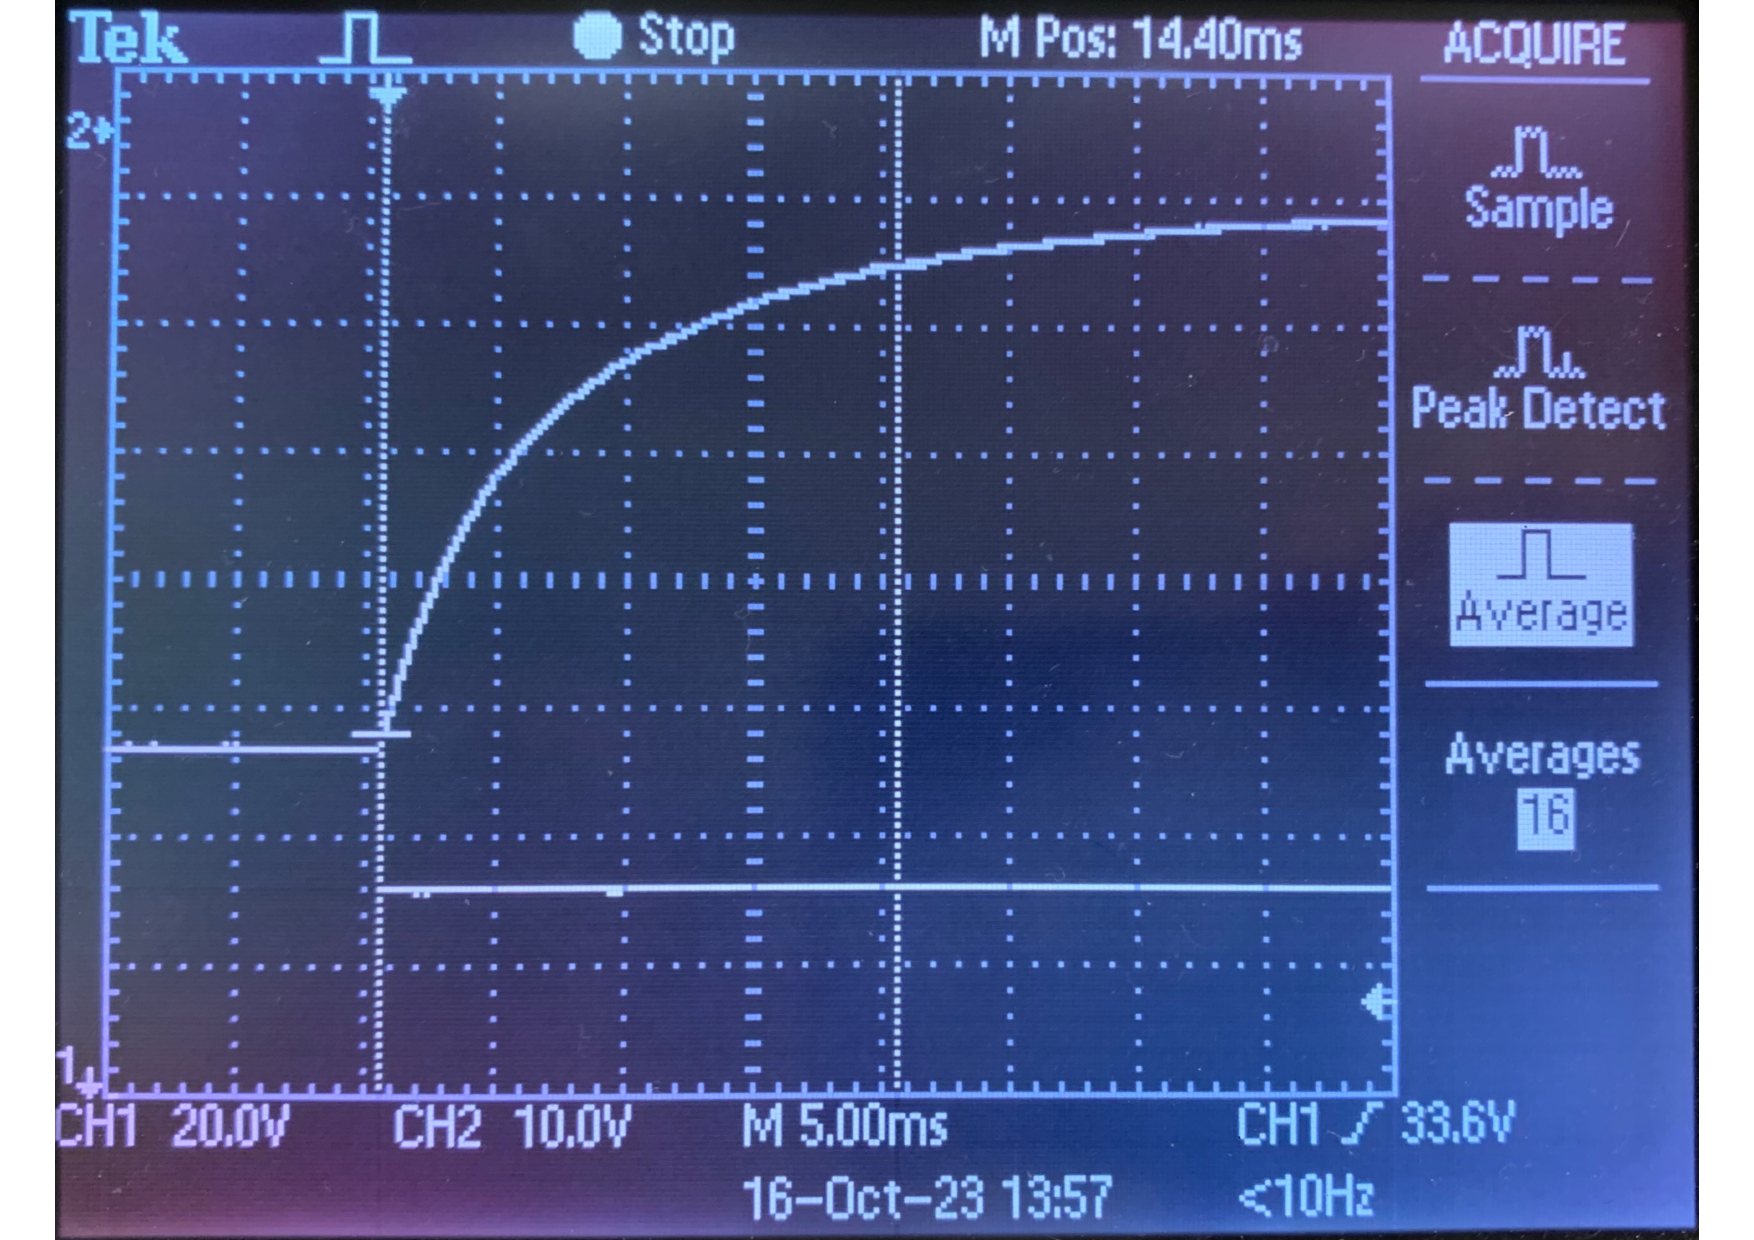
\includegraphics[height=9cm]{content/pics/ExpOszill.pdf}
  \caption{Bild des Oszilloskopschirms beim Auschalten des Magnetfelds. Gezeigt sind Werte für das 1. Isotop.}
  \label{fig:ExpOszill}
\end{figure}
\begin{figure}
  \centering
  \includegraphics{build/plot_exp.pdf}
  \caption{Messwerte für den exponentiellen Anstieg der Transmissionsamplitude $A$ aus \autoref{fig:ExpOszill} mit eingezeichneter
  Fitfuktion.}
  \label{fig:Exp}
\end{figure}

Die resultierenden Fitparameter sind in \autoref{tab:Exp} angegeben.
\begin{table}
  \centering
  \caption{Werte der Fits aus \autoref{fig:Exp} für die beiden Isotope.}
  \label{tab:Exp}
  \begin{tabular}{c l l l}
    \toprule
    {Isotop} & $a_{\text{max}} \mathbin{/} \unit{\volt}$ & $a_{\text{min}} \mathbin{/} \unit{\volt}$ & $b \mathbin{/} \unit{\per\second}$ \\
    \midrule
    1. Isotop & \num{40.5+-0.5} & \num{3.6+-1.0} & \num{137+-7} \\
    1. Isotop & \num{20.20+-0.33} & \num{-0.3+-0.4} & \num{166+-8} \\
    \bottomrule
  \end{tabular}
\end{table}
